\section{Implementierung}

In diesem Abschnitt wird die Struktur und Vorgehen bei der Erstellung der Implementierung geschildert.

\subsection{Architektur}

Die Implementierung wurde in mehrere Komponenten aufgeteilt. Diese sind überblicksartig in Abbildung \ref*{fig:compontents} einzusehen. \\
Die Module sind: \\

\begin{itemize}
    \item CarOfferTypes.elm
    \item DataHandling.elm
    \item Main.elm
    \item ParallelPlot.elm
    \item Scatterplot.elm
    \item StarPlot.elm
\end{itemize}

Im folgenden soll kurz auf die Implementierungen und derer Funktionen der einzelnen Module eingegangen werden. \\

\begin{figure}
    \centering
    \label{fig:compontents}
\end{figure}

\subsection{CarOfferTypes}

In diesem Modul wurden die verwendeten Typen definiert. Dazu gehören: CarOfferData, CarOffer und StarData, auf die eingegangen werden soll.

In Abbildung \ref{carofferdata} ist die Typdeklaration `CarOfferData` abgebildet. Dieser hält alle relevanten Daten für die Visualisierungen und wird innerhalb des Modells bei jeder Änderung geupdatet. \\
Es werden die Daten für alle Visualisierung und die aktuellen Zustände, der aktuell ausgewählten Parameter gehalten. \\

\begin{figure}[h]
    \centering
    \begin{mdframed}[backgroundcolor=black!10]
    \begin{minted}[fontsize=\footnotesize]{Elm}
        type alias CarOfferData =
    {
        data: List CarOffer
        , dataStarAvg: List StarData
        , dataStarSum: List StarData
        , yAxis : String
        , xAxis : String
        , firstCoordinate : String
        , secondCoordinate : String
        , thirdCoordinate : String
        , forthCoordinate : String
        , starParameter : String
    }
    \end{minted}
\end{mdframed}
\caption{CarOfferData Type}
\label{carofferdata}
\end{figure}

In Abbildung \ref{fig:caroffer} ist die Definition des CarOffer Typs zu sehen. Dieser dient dazu alle relevanten Attribute der Gebrauchtwagenanzeige typisiert zu halten. \\
\begin{figure}[H]
    \centering
    \begin{mdframed}[backgroundcolor=black!10]
    \begin{minted}[fontsize=\footnotesize]{Elm}
    type alias CarOffer =
    { brand : String,
    model : String,
    color : String,
    registration_date : String,
    year : Int,
    price_in_euro : Float,
    power_kw : Int,
    power_ps : Int,
    transmission_type : String,
    fuel_type : String,
    fuel_consumption_l_100km : Float,
    mileage_in_km : Float,
    offer_description : String,
    length_offer_description : Int
    }

    \end{minted}
\end{mdframed}
\caption{CarOffer Type}
\label{fig:caroffer}
\end{figure}

In der letzten Abbildung, Abbildung \ref{fig:stardatatype}, werden alle relevanten Attribute für den Starplot gespeichert. Dies ist nötig, da die benötigten Daten für den Starplot sich stark von denen, die für die anderen Visualisierungen, benötigt werden unterscheiden. \\
\begin{figure}[H]
    \centering
    \begin{mdframed}[backgroundcolor=black!10]
    \begin{minted}[fontsize=\footnotesize]{Elm}
type alias StarData =
    { brand : String,
    year : Float,
    price_in_euro : Float,
    power_kw : Float,
    power_ps : Float,
    fuel_consumption_l_100km : Float,
    mileage_in_km : Float,
    length_offer_description : Float
    }

    \end{minted}
\end{mdframed}
\caption{StarData Type}
\label{fig:stardatatype}
\end{figure}

\subsection{DataHandling}


\subsection{Main}

Innerhalb der Main-Komponente werden alle Funktionen der Subkomponenten aufgerufen und integriert.\\
Diese folgt einer so genannten Model-View-Update Architektur, wie in Abbildung \ref{fig:model-view-update} zu sehen.\\
Das Model kann dabei drei Zustände - Failure, Loading und Success - haben, wobei der Zustand Success zusätzlich als Parameter ein Objekt des Types CarOfferData (Abbildung \ref{carofferdata}) hat. Hier wird der aktuelle Zustand des Models hinterlegt.\\

\begin{figure}[H]
    \centering
    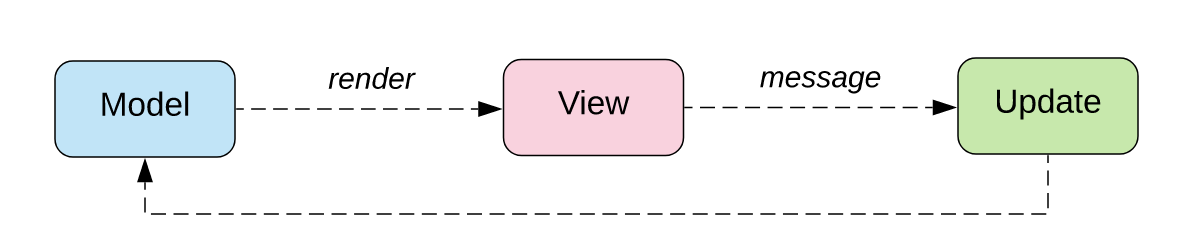
\includegraphics[width=\textwidth]{img/architecture.png}
    \caption{Model-View-Update Architektur}
    \label{fig:model-view-update}
\end{figure}

In der view-Methode werden die unterschiedlichen Zustände des Models verarbeitet und darauf basierend eine Ausgabe getätigt. Bei den Zuständen Loading und Failure, wird ein Platzhalter abgebildet und bei Success die eigentlich gewünschte Ausgabe. Dies ist ausschnittsweise in Abbildung \ref{fig:view-method}

\begin{figure}[H]
    \centering
    \begin{mdframed}[backgroundcolor=black!10]
    \begin{minted}[fontsize=\footnotesize]{Elm}
view : Model -> Html Msg
view model =
  case model of
    CarOfferTypes.Failure ->
      text "I was unable to load your book."

    CarOfferTypes.Loading ->
      text "Loading..."

    CarOfferTypes.Success fullText ->
      main_ []         -- Responsive fixed width container
        [ bootstrapCDN
          ,navigationBar
          ,topText
          , scatterPlotText

          ...
    \end{minted}
\end{mdframed}
\caption{Ausschnitt aus der view Methode}
\label{fig:view-method}
\end{figure}

In der update-Methode werden die Änderungen - aus Drop-Down-Menüs oder beim Laden von Daten - auf das Modell übertragen. Dazu werden hier unterschiedlicher Msg Typen unterschieden, die als Ereignisse agieren. \\
Diese werden mit einem case zugeordnet und dann basierend auf deren Parametern das entsprechende Teil des Models verändert. Eine Ausnahme bildet der "FetchData" Msg-Typ, welcher bei der Initialisierung ausgelöst wird. Hier wird das gesamte Model neu initialisiert. \\

\subsection{Scatterplot \& Parallelplot}

Diese beiden Komponenten werden hier gemeinsam aufgeführt, da sie aus den Übungen der Veranstaltung mit minimalen Änderungen übernommen werden konnten. \\
Die draw-Funktionen der Komponenten werden wie in Abbildung \ref{fig:aufrufe} in der view Funktion in Main.elm aufgerufen.
\begin{figure}[H]
    \centering
    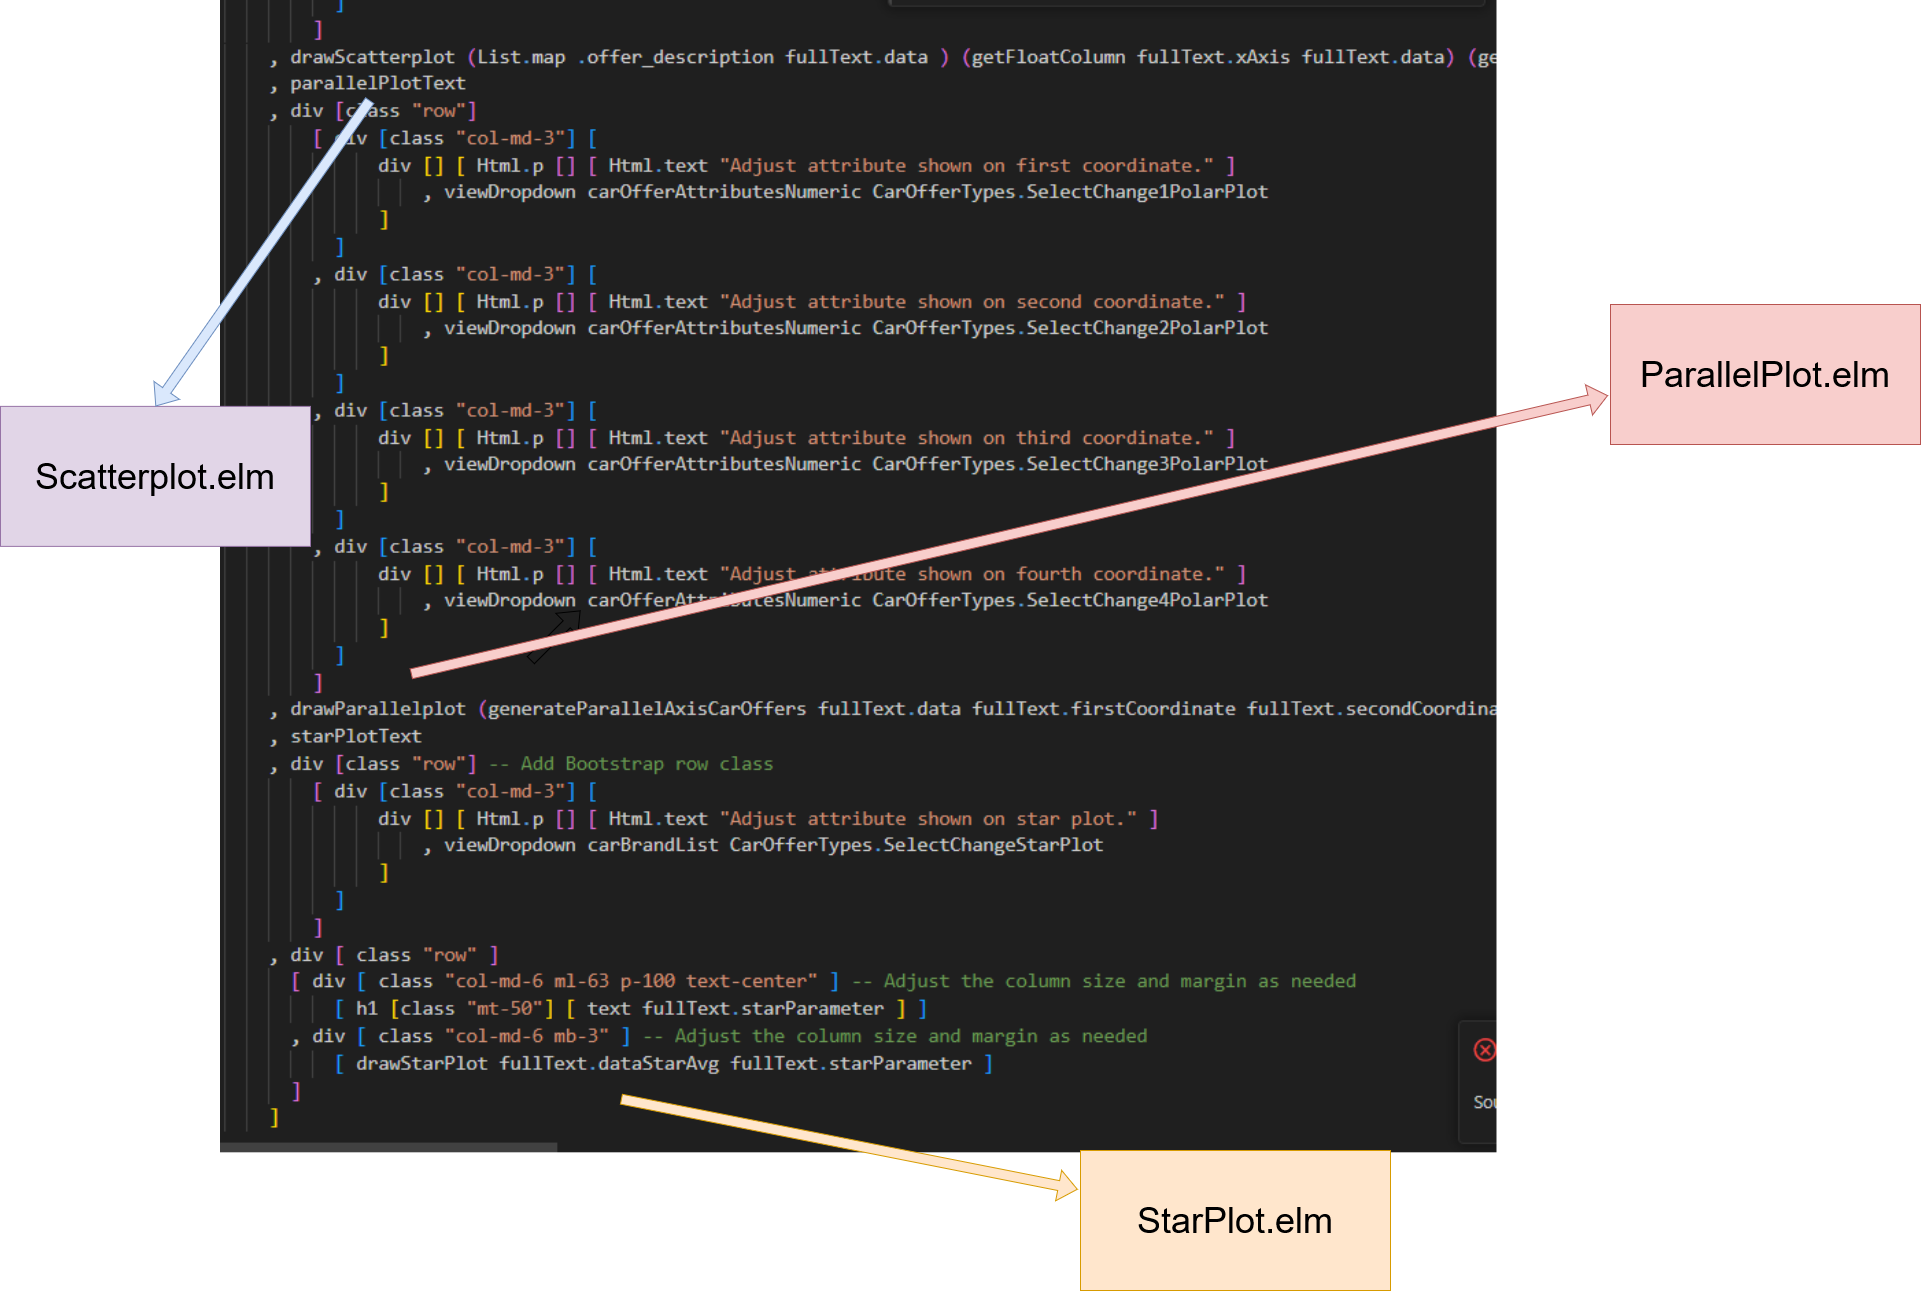
\includegraphics[width=\textwidth]{img/aufrufe.png}
    \caption{Aufrufe der Visualisierungskomponenten}
    \label{fig:aufrufe}
\end{figure}

\subsection{Starplot}